% Notas del integrante 1. Compilar notas/main.tex.
\section*{\personaUno · RPC}
\textbf{Proyecto}\quad \proyectoUno
\subsection*{Teoría y ejemplo sencillo}
\campo{Escribir lo que se dirá sobre RPC, el contrato, la entrada y la salida de la demo.}
\espacio
\subsection*{Aplicación futura al proyecto}
\campo{Explicar el estado actual y qué servicio se implementaría. Añadir la operación, motivación, transparencias, CAP/PACELC y comparación con fuentes.}
\espacio
\subsection*{Fallo supuesto y conclusión}
\campo{Describir causa, impacto, detección, recuperación propuesta y prueba de validación.}
\espacio
\textbf{Bosquejo a mano}\quad
\begin{center}
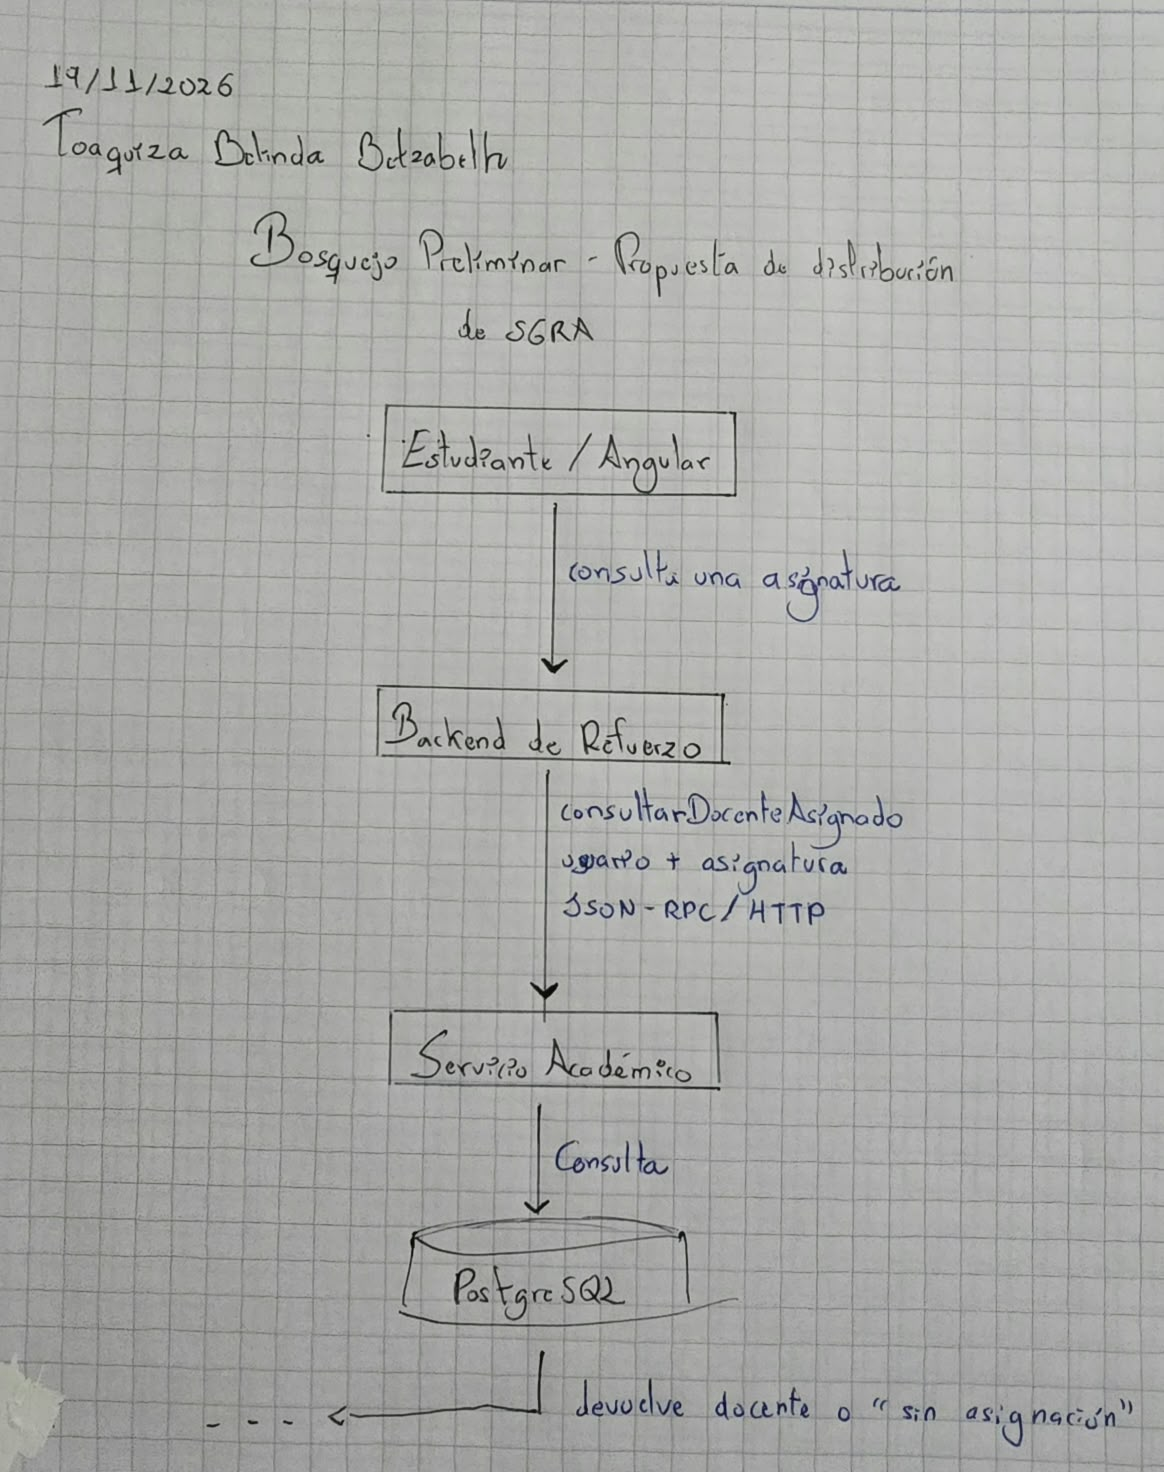
\includegraphics[height=.30\textheight,keepaspectratio]{../evidencias/Belinda T/esquema-mano/sgra-bosquejo-preliminar-consulta-docente-belinda-2026-11-19.jpeg}
\end{center}
{\small Bosquejo original de Belinda Toaquiza, 19 de noviembre de 2026. El diagrama formal precisa los límites de proceso, la identidad autenticada y el retorno de las respuestas. La consulta académica separada es una propuesta futura.}
